\documentclass{article}

\usepackage[T1]{fontenc}
\usepackage{graphicx}
\usepackage[a4paper, margin=2cm]{geometry}
\usepackage{hyperref}
\usepackage{lastpage}
\usepackage{fancyhdr}
\usepackage{datetime}
\usepackage{glossaries}
\usepackage{xurl}

\hypersetup{
  colorlinks = true,
  urlcolor = blue,
  citecolor = black,
  linkcolor = black
}


\makeglossaries

\newglossaryentry{gmp}
{
  name=GMP,
  description={Good manufacturing practice}
}

\newglossaryentry{fdg}{name={FDG},description={[$^{18}$F]Fluorodeoxyglucose, a
common radioactive tracer used for PET images}}

\newglossaryentry{CIMT}{name={CIMT},description={Center for IT and Medico
technologies. Responsible department for IT in the Capital Region of Denmark}}

\newglossaryentry{git}{name={Git},description={Git is a free and open source
distributed version control system designed to handle everything from small to
very large projects with speed and efficiency. Found at
\url{https://git-scm.com}}}
\newglossaryentry{invalid state}{name={invalid state},
description={This is a database}}

\newglossaryentry{ema}{name={EMA}, description={European medicines Agency -
\url{www.ema.europa.eu}}}

\newglossaryentry{invalid data}{name={invalid data},description={Nonsensical
data that could never be valid. Examples include a reference to an nonexistent
object or Negative halflife or activity}}
\newglossaryentry{incorrect data}{name={incorrect data},description={Data that
 doesn't reflect reality. Examples include a misspelled batch number or an
  activity entry which does not match actual activity in the vial}}

\graphicspath{{./figures/}}

\fancyhf{}
\fancyfoot[L]{\today}
\fancyfoot[R]{Page \thepage \, of \pageref{LastPage}}
\fancyhead[L]{Technical documentation \& Risk assessment of Tracershop}
\fancyhead[R]{Doc nr: <I'm a document Number>}
\pagestyle{fancy}

\author{Christoffer Vilstrup Jensen}
\title{Technical documentation}
\begin{document}


\begin{titlepage}
  \begin{minipage}{0.48\linewidth}
    
\includegraphics[width=0.6\linewidth]{logo.png}
  \end{minipage}
  \begin{minipage}{0.48\linewidth}
    \raggedleft
      
\includegraphics[width=0.6\linewidth]{petlogo_small.png}
  \end{minipage}
  \vspace{1cm}
  \begin{center}
    \Huge Technical documentation and risk assessment for Tracershop \\
    \vspace{1cm}
    \Large Christoffer Vilstrup Jensen\\
    MSc. Computer Science\\
  \end{center}
\end{titlepage}

\section*{Introduction}

This document describes the electronic web shop, Tracershop, used for ordering
and release of radioactive tracers for clinical procedures and radiochemistry
produced at Rigshospitalet's Cyclotron unit. Since radioactive tracers are
medicinal products, Tracershop must fulfil documentation requirements stated by
GMP Volume 4 annex 11, which this document describes.\\
Rigshospitalet delivers radioactive PET tracers to hospitals and scientific
institutions around Copenhagen. It would not be possible to perform PET scans
without these tracers. Therefore Tracershop should be considered a important
piece of software.\\
Tracershop was released in 2004 and is used to this day. Due to it's age a new
system have been developed with the intent to replace the old system. This
document contains a short description of the old system, then a deeper
explication of some techniques and technologies that the system is using to
obtain a "Better" software product.\\
Since annex 11 is dated, \gls*{ema} has released a concept paper on annex 11\footnote{
\url{https://www.ema.europa.eu/en/documents/regulatory-procedural-guideline/concept-paper-revision-annex-11-guidelines-good-manufacturing-practice-medicinal-products_en.pdf}}
containing various comments on the guidelines presented in annex 11.
These comments have also been considered when applicable. \\
The document have been review with Jacob Madsen and Helle Østergren Bak as
Process owners, and Christoffer Vilstrup Jensen as developer.

\subsection*{User Requirements}

The requirements of the software, that tracershop fulfils are:

\begin{itemize}
  \item A shop user can order radioactive tracer on behalf of a customer,
  which have been certified to the ordered tracer.
  \item A shop user can view any order that been have made to a customer they
  are associated with. \\
  They can view batch numbers of any product that they have received. \\
  They can delete orders, that have been requested, but not accepted or
  released.\\
  They cannot alter accepted or released orders.\\
  They cannot view orders from users that they are not associated with.
  \item A production user, that have been certified can release a radioactive
  tracer.
  \item Production admin can grant and remove certification of other production
  users. A production admin user cannot grant any rights to themselves.
  \item A released order has a batch number and a record of who released it.
  \item Non authenticated users cannot alter or view information in tracershop.
  \item A released tracer must display if it's intended for preclinical usage or
  human usage.
\end{itemize}

\subsection*{Terminology}

Tracershop handles two different types of orders. Activity based orders and
Injection based orders.\\
An \textbf{activity order} is defined as: An order, where a customer orders an
amount of MBq radioactive tracer at a predetermined time slot known as a
"deliver time".
It's the user responsibility to account for radioactive decay between injection
time and delivery time. Delivery time slots are determined by the production
users and are allocated per user.\\
An \textbf{injection order} is an order with a number of injections with a
predefined amount of activity, and it's Tracershops responsibility to account
for any radioactive decay between production time and injection time.\\
Users er limited which injection tracers they can order, determined by the
production users.

\section*{Tracershop - Current system}

The software ecosystem is centered around a MySQL 5.1 database running on a
openSUSE 11.2 distribution, which contains all the records and logs about the
production of tracers. This database is back up on an external machine every day
at midnight.

Tracershop is a web site hosted with Zope 2-2.13 web interface at
\url{http://pet.rh.dk} allowing the users to systematically write to the main
database. These messages are logged.\\
The website is deprecated and no longer receive updates.
The system contains an dispenser, that records how much radioactive material was
dispensed, allowing accurate tracking of activity in vials and minimizing human
error. This data is pushed via a script to tracershop.\\
An overview of the current system can be seen in figure \ref{fig:oldsys}.
\begin{figure}[ht]
  \begin{center}
    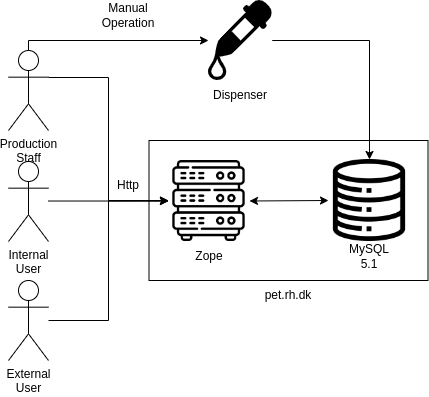
\includegraphics[width=0.6\linewidth]{OldSetup.png}
    \caption{Current Tracershop system}
    \label{fig:oldsys}
  \end{center}
\end{figure}

The system is hosted on internal server owned by The Department of Clinical
Physiology and Nuclear Medicine. This is not desired because hosting server is a
core task for \GLS{CIMT} and not for the clinical departments.

\subsection*{Database layout}
The database contains the following tables:
\begin{enumerate}
  \item Log - Likely Zope related. No longer in use as the last entry was in
  2010-03-18.
  \item MiscData - Likely Zope related. Likely a temporary value container.
  \item Roles - Zope related, defines different user roles in the Tracershop
  program.
  \item Sessions - Likely Zope related, defines active user sessions.
  \item Tokens - Likely Zope related, Likely defines the length of active
  sessions.
  \item TracerCustomer - Defines which user have access to order which injection
  Tracer.
  \item Tracers - Catalog of tracer available in tracershop.
  \item UserRoles - Relates user to a Role from the Role table.
  \item Users - All users able to be authenticated in tracershop
  \item VAL - Record of a vial with tracer, produced by the dispenser.
  \item VAL2 - Not in use.
  \item blockDeliverDate - Extraordinary dates where tracershop is closed, such
  a holydays.
  \item deliverTimes - Weekly points in time specifying when a customer can
  place an activity order.
  \item isotopes - Catalog of radioactive isotope used in the tracers.
  \item orders - List of activity orders.
  \item productionTimes - Weekly points in time, where a production should
  happen. Entries are also referred as a run.
  \item productions - Production of tracers.
  \item storage - Old mails, assumed not in use.
  \item t\_orders - List of injection orders.
\end{enumerate}

The database is not utilizing the foreign key restriction, meaning that the
relations are ensured at application level and not the database level, and as
 such only reaches the first level of database normalization.
This low level of normalization allow a number of error to be present in the
database:
\begin{itemize}
  \item Reference errors - When a field references another table without the
  foreign key restriction, then the reference can point an entry that doesn't
  exists, which is a error, therefore any change to an ID, must by application
  logic update the rest of database.
  \item Transitive functional dependencies may not respected. As an example:
  An activity order contains both the amount of radioactive material was ordered
  and how much tracer should be produced while taking into account the overhead
  percentage of the customer. If the ordered amount is edited then the database
  integrity relies on application logic to update overhead amount.
\end{itemize}
It's considered an industry standard to keep databases in third normal form,
which require the database to be designed in such a way, that these errors
cannot occur.

\section*{The new Tracershop}
For the rest of the document, the name Tracershop will refer to this solution.
The setup for Tracershop can be seen in figure \ref{fig:TSO}.
It's a virtual computer hosted by \gls{CIMT} running Red hat 8
\url{https://www.redhat.com/en}:

\begin{figure}[ht]
  \centering
  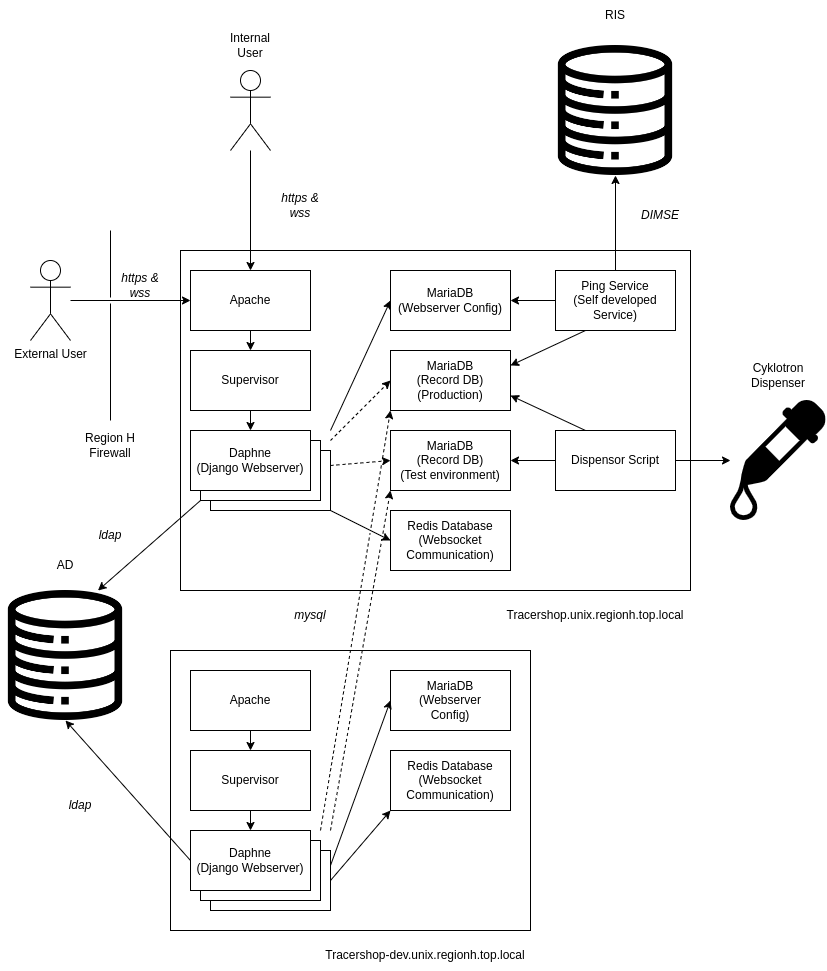
\includegraphics[width=0.6\textwidth]{figures/TracershopSystemOverview.png}
  \caption{The new system}
  \label{fig:TSO}
\end{figure}

\begin{itemize}
  \item[] plnxtshop01.unix.regionh.top.local - 10.146.12.175
\end{itemize}
The server run the following programs:

\begin{itemize}
  \item F5 - This is reverse proxy web service, managed by Net design. It's
  responsible for forwarding http and ws request to Tracershop.
  \item Apache - open source web server, \url{https://www.apache.org}
  \item Daphne - Websocket protocol server, developed for django channels
  \url{https://github.com/django/daphne}
  \item Vial Fetcher Service - This is a small program responsible for fetching
  data from the dispenser, however since the dispenser is only able to dispense
  files, a network drive is an intermediate link.
  \item MariaDB - Open source Mysql database - \url{https://www.mariadb.org}
  \item Redis Database - Open source in memory database - \url{https://www.redis.io}
  \item Supervisor - Monitor program for Daphne \url{http://www.supervisord.org}
  \item Ping Service - This is a hl7 message server, that will receive bookings
  with relevant tracers, this allows shop users to automatically order tracers
  based on incoming bookings.
\end{itemize}
The underlying web service is an open source django / channels web server found
at \url{https://github.com/demiguard/Tracershop}. It's developed and maintained
by Christoffer Vilstrup Jensen.

The tracershop uses common software packages for web servers:
\begin{itemize}
  \item React - Frontend Javascript library developed by facebook.
  \url{https://reactjs.org}
  \item Django - Backend Python web server library
  \url{https://djangoproject.com}
  \item Channels - Django extension for using websockets.
  \url{https://channels.readthedocs.io./en/stable}
\end{itemize}
These packages are well supported and all in active development,
so their developers will continue to provide security updates.
Because these packages are commonly used, it's easy to find a replacement
developer, should the current developer leave Rigshospitalet.

\subsection*{Message handling}
Tracershop utilize websockets instead of purely http communication,
because websockets allows the server to push updates to the users unprompted,
because the protocol uses a persistance connection, while http does not use a
persistent connection. This technology allow the communication protocol seen in
figure. \ref*{fig:websocketMessage}

\begin{figure}[ht]
  \begin{center}
    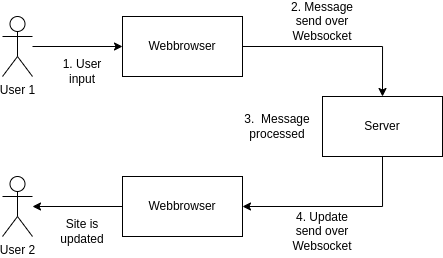
\includegraphics[width=0.6\linewidth]{websocketMessage.png}
    \label{fig:websocketMessage}
    \caption{Overview of the message handling.}
  \end{center}
\end{figure}

\begin{enumerate}
  \item A user causes an update, that needs processing from the server.
  \item A message is send by the server
  \item The message is processed by the server
  \item the server sends a responses, that the message have been processed. If
  the message type require an update websites state, then the server informs
  all clients by broadcasting the message.
  \item The server rerenders the website with the modified state in mind.
\end{enumerate}

To ensure that each message is valid, and that user is authorized to send that
message, all message are processed in a three step plan seen in figure
\ref*{fig:messageHandle}

\begin{enumerate}
  \item Validate message - The server determines if the message has all the
  needed fields and that the fields contains values of the expected type. It
  also ensures that sender doesn't have an outdated version of the frontend
  client. If validation fails, there's no update to the database.
  \item This checks that the sender is authorized to send, this message type.
  If authentication fails, there's no update to the database.
  \item Message processing, this step performs the message.
\end{enumerate}

\begin{figure}[ht]
  \begin{center}
    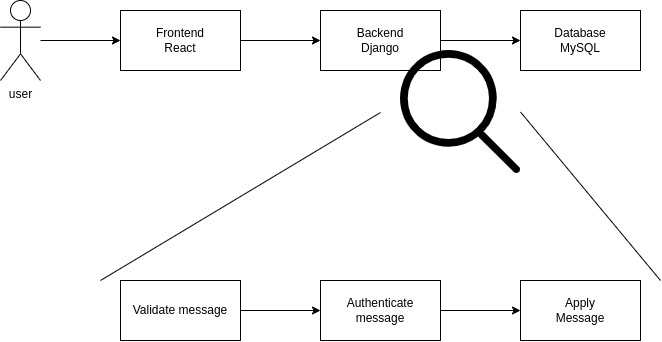
\includegraphics[width=0.6\linewidth]{MessageHandeling.png}
    \caption{Message handling by the backend}
    \label{fig:messageHandle}
  \end{center}
\end{figure}

\subsection*{New login system}

The new tracershop system uses an external authentication system, provided by
the Capital region called BAM ID, managed by \GLS{CIMT}. All members of staff
working in the capital region have a BAM ID login.

This login have various security features build in, such as automatic
deprecation of passwords, password reset, deactivation of inactive accounts, and
minimum complexity requirements to passwords. \GLS{CIMT} also handles
reestablishment of forgotten passwords.
Secondary tracershop doesn't need to store passwords and instead store tokens
that the system can authenticate against CIMTs systems.Consequently if the
system is compromised, no data about the users passwords can be leaked.

All users in Tracershop are personal and have a role determining their
rights. A user can only have a single role.
These roles are divided into a Shop- or Production category. Shop users are
representatives for a customer organization, that uses products from Tracershop.
Production users are members of Rigshospitalet Cyclotron unit and releases
tracers in tracershop.

If a user is a staff member of the Capital region they acquire their role by
contacting the local active directory manager (CBAS administrators), requesting
the role. The manager can then determine if the role that is requested is
appropriate and accept or deny the request based on their judgement.

All the roles are as follows:

\begin{itemize}
  \item Shop - External - This user is related to a customer, which is not part
  of the capital region. The user isn't an employee of the Capital region and
  doesn't have BAM ID, therefore their profile cannot be managed by CIMT or
  benefit from automatic ordering.
  They can view their assigned customer's orders and order tracer authorized to
  the customer.
  Each of these user are connected to an external customer. The user is managed
  by an production admin.
  \item Shop - Internal - This is an employee of the Capital region and
  therefore have a BAM ID. A user is associated with one or more internal
  customers. This user is managed by a "Shop Superuser" user.
  \item Shop - Superuser - This is an internal shop user with additional rights
  to modify the automatic generated order based on a RIS booking.
  They can grant an internal user access to the same customers that they
  moderate.
  \item Production - User - The user can view and accept orders from all
  customers. They can release tracer of authorized types.
  \item Production - Admin - Everything the production user can. Grant release
  rights to other production users, create new tracers, allow tracers to ordered
  by customers, and manage external user.
  \item Site Admin - The equivalent of a root user. The user can mimic all the
  functionality of other roles. The user isn't intended to use tracershop only
  to support it.
\end{itemize}

In addition to the user role, tracershop keeps track of which user can represent
which user. If a shop admin user represent a customer, they can grant other
shop internal users the right to represent this customer.


\subsection*{Logging}
Annex 11 is very light on it's requirement of logging, therefore we refer to the
comments in the concept paper. (ref?)
The raw logs are only accessible by system administrators. Each log entry has a
time stamp, and a record of the user which invoked the user statement.
Anonymous users cannot trigger log actions, because they are filtered away by
the F5 reverse proxy.\\
The new tracershop contains the following logs:
\begin{itemize}
  \item Audit log: The audit log contains significant actions related to GMP.
  The log is permanent (not rotating), and is backed up at the same level as the
  server. The following actions are log in the audit trail:
  \begin{itemize}
    \item The system automatically assign or reassigns: the Shop Admin, Production Admin, or
    Site Admin user group to a user.
    \item A production user / admin manually adds a vial, data of the vial is
    logged.
    \item A production user / admin manually edits an existing vial, the old and
    new data is logged.
    \item A production user / admin releases an order.
    \item A production user / admin edits a released order. The old and new
    order data is logged.
    \item A production admin / Site Admin grants releasing rights to a
    production user.
  \end{itemize}
  \item Operational web service Log: General operational messages - Indented for
  debugging. Weekly Rotating log, 4 weeks of logs are kept.
  \item Operational ping service logs: Logs generated by the ping service.
  Weekly rotating log, 4 weeks are kept.
  \item Operational Vial fetcher service logs: Logs generated by the vial
  fetcher service. Weekly rotating log, 4 weeks are kept.
\end{itemize}


\subsection*{Correctness of Tracershop}

Ensuring correct behavior of any program is a difficult process. Errors increase
proportional to the complexity of the system, interactions with other systems
and changes to the software ecosystem.\\
To combat errors an automated test suite have been developed. These tests can be
divided into three parts, an predefined arrange state, an action to be performed
and finally an assertion about the result of the action.\\
A well developed test suite has the benefit of making changes easier to
implement correctly because they display any cascading impact of any changes.\\
A test covers a line of code if that line of code is executed in the test. From
this term coverage of a test suite is defined as the percentage of lines covered
by all tests of the suite.\\
Recommended percentage of code coverage is a greatly debated topic in the
software development communities. The main debate revolves around the last 5-10
percentage points of code coverage. This is because these lines of code often
handle edge cases, are unreachable or handle faulty connections to other sub
systems.\\
High code coverage can also lead to rigid code bases, slowing down development
of new features. Full test coverage doesn't prevent software related errors from
occurring. Tests are also not free, as they take time to develop and maintain.
The author recommend a 90 percentage code coverage.

Software tests doesn't reduce human errors, but can be reduced by various sanity
checks, that can be performed automatically. Nor does they prevent other
subsystem from failing.

\section*{Risk assessment}

Tests can by definition only showcase that the program works in a predefined
"idealized" environment nor do they deal with incorrect data.
To combat the problems uncovered by the automated testing. There has been made a
risk assessment below.\\
A risk assessment is a collections of risks, where each risk consists of:

\begin{itemize}
  \item A description of the risk.
  \item A highlight of the current system
  \item A likelihood of how likely an incident is to occur.
  \item A damage estimate of an incident.
  \item A plan of action if an incident happen.
  \item How the new system reduces this risk
\end{itemize}

This risk assessment doesn't include production related risks such a dropped
vial, or tracers not passing quality control.\\
The dispenser and the program transferring data have not modified by the new
Tracershop, and therefore derives its validity from previous risk assessments.
See document number.: PVP-PROD-Tracershop-001-14.01 in D4, for the latest
validation of Tracershop.

\begin{itemize}
  \item Loss of a server.
  \begin{itemize}
    \item[Description] - A hosting server might become unavailable for of number
    a reasons:
    A foreign threat might encrypt the entire server, hardware failure, or a
    critical files might become corrupted due to aging hard drive.
    This is not an exhaustive list of reasons for server loss however other
    factors have minimal likelihood.
    It's beneficial to have plan of action in the event of an incident caused by
    an unknown risk.
    \item[Currently] - Currently the service runs on old hardware, insecure
    protocols and outdated software, which raises the likelihood of an incident
    occurring.
    \item[Likelihood] - Low to medium, Likelihood is increasing with age of the
    system.
    \item[Damages] - High - Without the server, it would be impossible to create
    electronic records of produced tracers.
    \item[Plan] - Repairing the server hardware might be possible and could
    restore the system to a pre-incident state, within 1-5 working days.
    If that's not possible to repair a new server is required. Assuming that the
    system is not deployed on \GLS{CIMT}s services and a spare server is not
    available, procuring a new server would take between 4-12 weeks with a 1
    week installation period afterwards.\\
    Any data not in the backup would be lost.
    \item[New System] - The system is hosted by CIMT, in a virtualized
    environment, allowing for easy cloning and therefore a short the recovery
    period.
  \end{itemize}
  \item Database is brought into an invalid state or incorrect state.
  \begin{itemize}
    \item[Description] - Due to the fact that it's the application
    responsibility to ensure correctness of the database, this is a risk of
    incident.\\
    If the record database is in an invalid state, undefined behavior might
    occur because some data is invalid.\\
    Consider an example where a tracer is deleted. All orders with that tracer
    can no longer be determined to be of that tracer.\\
    A common source of errors have been duplicate acceptance messages, this have
     causes orders appear released. In the new tracershop, both accepting and
     releasing orders are idempotence operations.
    \item[Currently] - If the database is in an invalid state, the site is
    unavailable.
    \item[Likelihood] - Low - The web services doesn't allow, the user to
    perform arbitrary SQL queries,
    only predefined queries that take the database from one valid state to
    another valid state.
    It's difficult to ensure all possible user inputs, so it's possible that a
    user query might bring the database into an invalid state.
    An incident could occur if a system administrator creates a query that
    brings the database is into an invalid state.
    \item[Damages] - None to Low - Restoring the database is an easy task for a
    system administrator, worst case would be to revert to a backup.
    If the invalid state persist unnoticed for more 1 day the backup will be
    over written and the damage made permanent.
    \item[Plan] - Upon notice a system administrator would enter the database
    and create a query to revert the database into a valid state.
    All queries made by tracershop to the record database is logged, which can
     greatly help system administrator to undo the damage.
    If the system administrator unable to restore the data using a query, then
    the plan switches to rollback to a backup of the record database, causing 1
    days worth of data loss.\\
    Note that direct queries to the database is not logged to the audit log,
    therefore their actions are untraceable, similarly their edits might not
    record the previous data, that is required to be logged.
    \item[New system] - A new database has been designed to be on fifth normal
    form, eliminating reference and transitive errors, making it impossible to
    bring the state in an invalid state. A page for unexpected errors has been
    created, giving some hints to what the error might be.
  \end{itemize}
  \item Incorrect user input
  \begin{itemize}
    \item[Description] - Tracershop have a number of fields, where the user must
    write some data in. Most critically this includes batch numberBecause it's
    humans that write this data, the system is subject to human error.
    It's incredible difficult to prevent this as there's nothing inherently
    wrong with \gls{incorrect data} user input. This also includes whenever a
    user forgets to update a piece of data.
    \item[Currently] - No warnings are given when attempting to release an order
    from another day.
    \item[Likelihood] - High. Humans use this program, no further
    elaboration required.
    \item[Damages] - None to High - Not all data in tracershop is critical,
    however if incorrect batch number is written to the database and the error
    is not noticed, then that could put patient safety at risk. If the incorrect
    data is auxillary, then there's no damages.
    \item[Plan] - If the data is committed, a system administrator must edit the
    data, if not the data can be edited in tracershop. The new system allow user
    to edit incorrect of non critical entries.
    \item[New Systems] - Additional warning has been made for commons errors,
    like freeing orders from the wrong date. See figure \ref{fig:dayhint}.

    \begin{figure}[ht]
      \begin{center}
        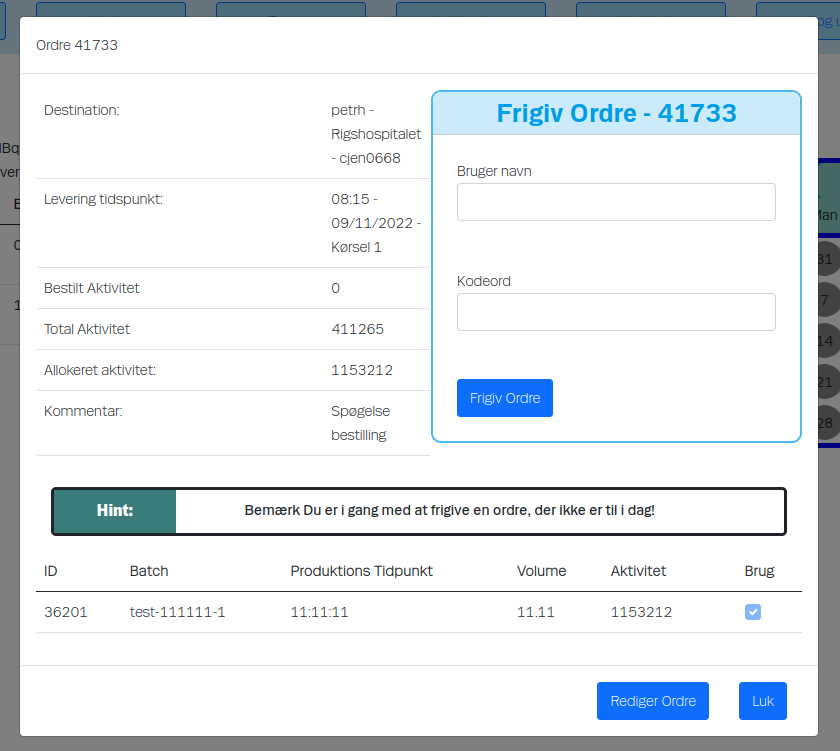
\includegraphics[width=0.6\linewidth]{figures/DayHint.png}
      \end{center}
      \caption{Modal for releasing an order}
      \label{fig:dayhint}
    \end{figure}

  \end{itemize}
  \item The dispenser script stops working
  \begin{itemize}
    \item[Description] - The service that provides information on the tapped
    vials consists of many different machines which introduces some fragility,
    as if any of the links of the chain fail, the entire service fails.
    These are:
    \begin{itemize}
      \item The computer connected to the dispenser
      \item CIMT network drives.
      \item The Tracershop main service.
    \end{itemize}
    \item[Currently] - The current system only allows for the dispenser to be
    used with FDG, the new system can use this system any number of tracers.
    \item[Likelihood] - Low - While there's many links, two of them are of high
    reliability. Namely the network drive and the web hosting server. These
    servers are prioritized by CIMT to keep up.
    The final computer is connected to the dispenser. While it's unlikely to
    fail without changes, however if this PC would become a CIMT controlled PC,
    then it would be subject to various updates, that might break the programs
    running on the PC. If the computer controlled by CIMT likelihood increase to
    medium.
    \item[Damages] - Low - Vial data can be written by human. This introduces
    human error and falls in under the risk of human error.
    \item[Plan] - Users would be forced to manually input data, that normally
    would have been transferred automatically and correctly.
  \end{itemize}
  \item Email server is unavailable
  \begin{itemize}
    \item[Description] - The email service is external, thus may for any reason be unavailable for an undefined amount of time.
    \item[Likelihood] - Unknown - The author have so limited experience with the available of the mail server, that a valid likelihood estimate is difficult to make.
    \item[Damages] - None to low - Customers are required to wait for confirmation that the tracer passed quality assurance mandated by \GLS{gmp}, so if the email server is down, the customer can not be notified through email.
    \item[Plan] - Delivery bills can be send via mails, phone calls and other communication.
    \item[New system] - The users can download delivery bills in new system, emails are deprecated and will shut down.
  \end{itemize}
  \item Malicious usage of tracershop
  \begin{itemize}
    \item[Description] - A user of tracershop attempt to sabotage the site. This risk also includes impersonation of staff members.
    \item[Currently] - All communication is unencrypted, the service is vulnerable to SQL injections.
    \item[Likelyhood] - Minimal - Users both staff and customers are verified users, which minimizes the risk of malicious usage.
    \item[Damages] - Low - Even in the event of that a user some how manages to destroy the record database, the backup is stored externally and thus not subject to any attack by the malicious user.
    \item[Plan] - All account are Personal. Critical actions such as freeing orders are audit logged. Allowing system administrator to identify the malicious user.
    There's a detection of SQL injections before the execution of each query, if it detects an injection it discards the query.
    \item[New system] - Security holes with SQL injections are patched. Communication is sent over encrypted channels.
  \end{itemize}
\end{itemize}


\section*{Conclusion}

The new system contains substantial upgrades to user experience, IT security,
and functionality. It fulfil the requirements stated by GMP Volume 4 Annex 11


\clearpage

\printglossary[type=main,style=long,nonumberlist]

\clearpage

\section*{Appendix}

\begin{figure}[ht]
  \begin{center}
    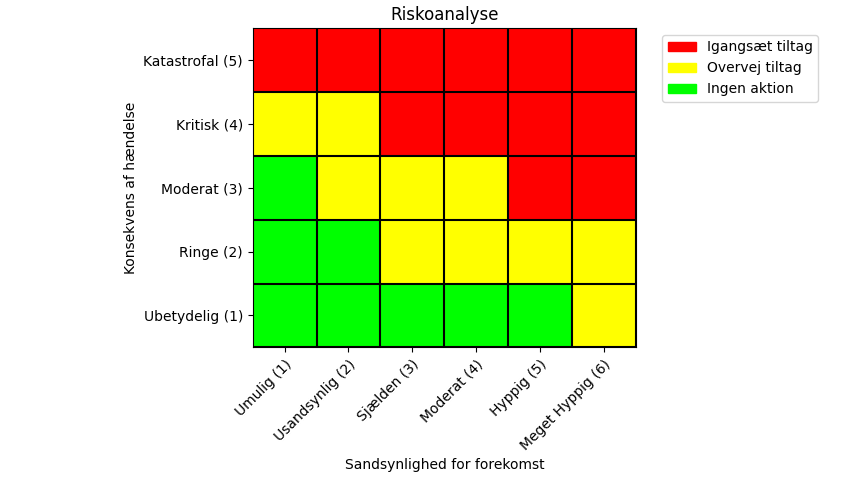
\includegraphics[width=\textwidth]{figures/risk_analyse.png}
  \end{center}
\end{figure}
\end{document}
